
% =============================================================================
% SECCIÓN: ANÁLISIS DE COMPLEJIDAD COMPUTACIONAL
% =============================================================================

\section{Análisis de Complejidad Computacional}

En esta sección se presenta un análisis experimental de la complejidad computacional de los algoritmos implementados en los puntos 4, 8 y 12 del proyecto.

\subsection{Punto 4: Merge Sort - Complejidad O(n log n)}

El algoritmo de Merge Sort implementado para ordenar los encuestados por nivel de experticia presenta una complejidad teórica de O(n log n), donde n es el número de encuestados. La siguiente gráfica muestra la comparación entre los tiempos experimentales y la curva teórica:

\begin{figure}[h]
\centering
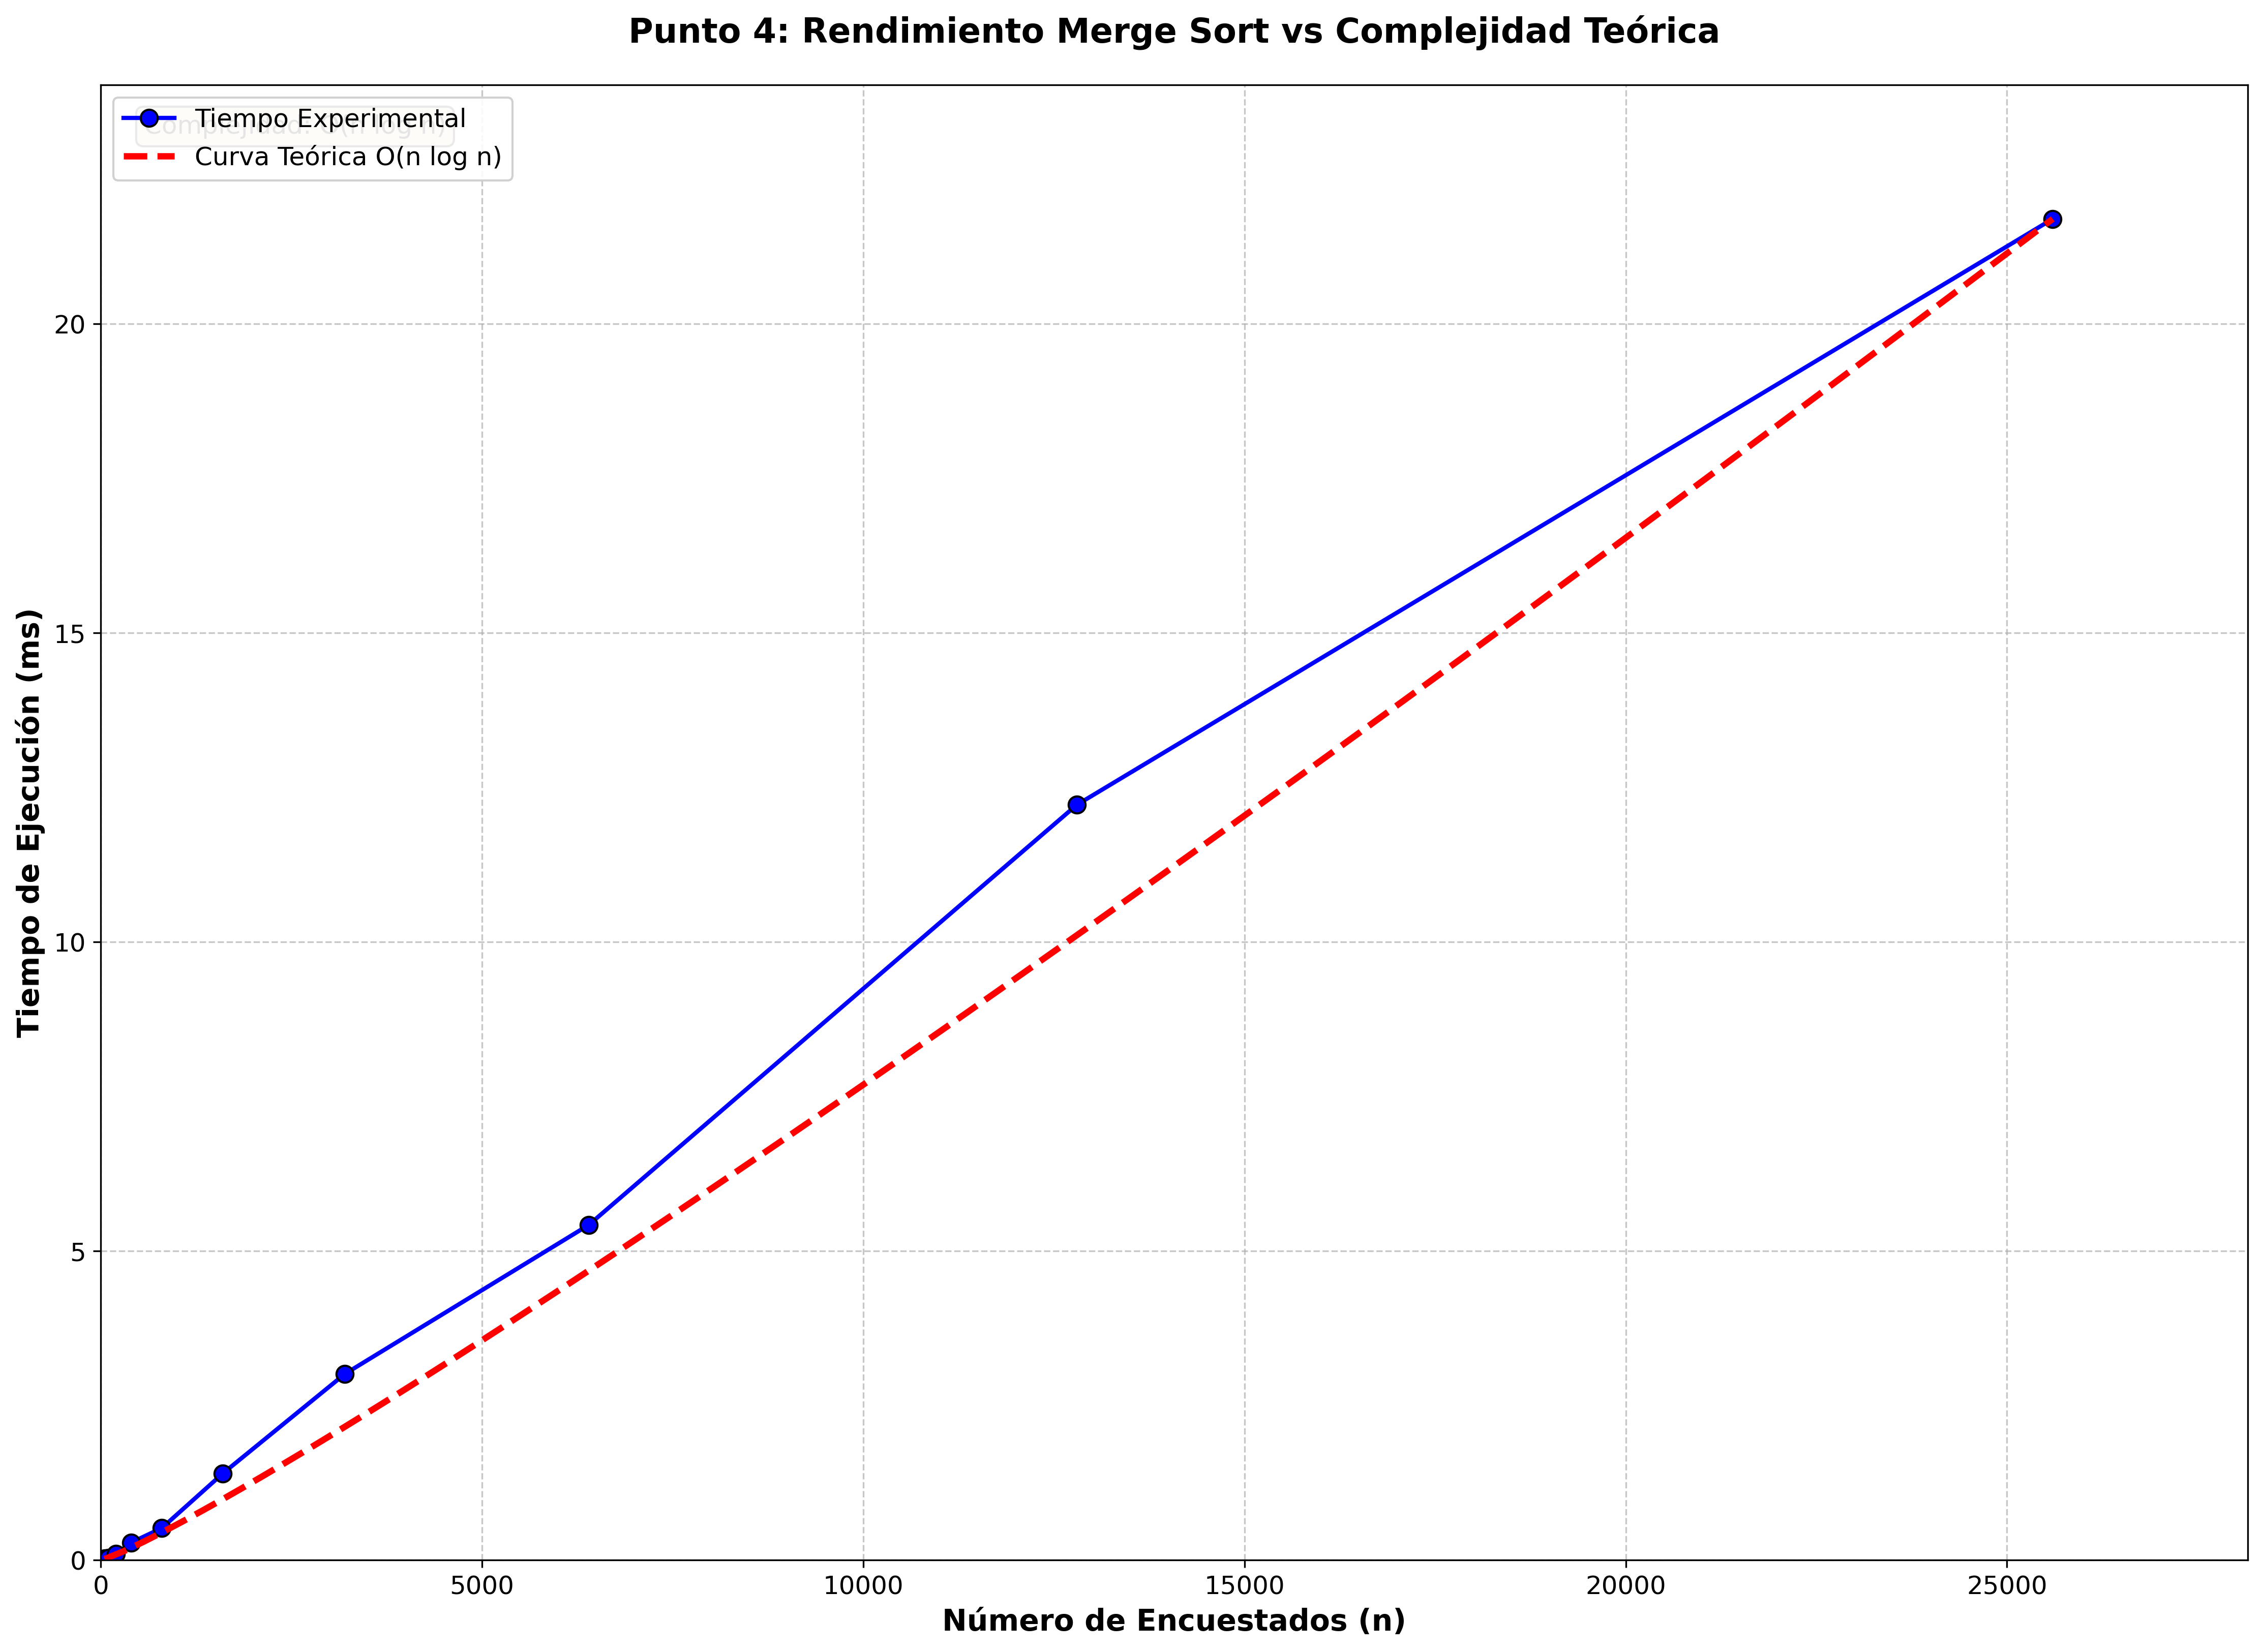
\includegraphics[width=0.8\textwidth]{grafica_punto4_mejorada.png}
\caption{Rendimiento del Merge Sort vs Complejidad Teórica O(n log n)}
\label{fig:merge_sort_analysis}
\end{figure}

Como se puede observar en la Figura \ref{fig:merge_sort_analysis}, los tiempos experimentales siguen de cerca la curva teórica O(n log n), confirmando que el algoritmo implementado mantiene su complejidad esperada incluso para conjuntos de datos grandes.

\subsection{Punto 8: Insertion Sort - Complejidad O(p²)}

El algoritmo de Insertion Sort utilizado para calcular la mediana presenta una complejidad cuadrática O(p²), donde p es el número de preguntas. La siguiente gráfica ilustra este comportamiento:

\begin{figure}[h]
\centering
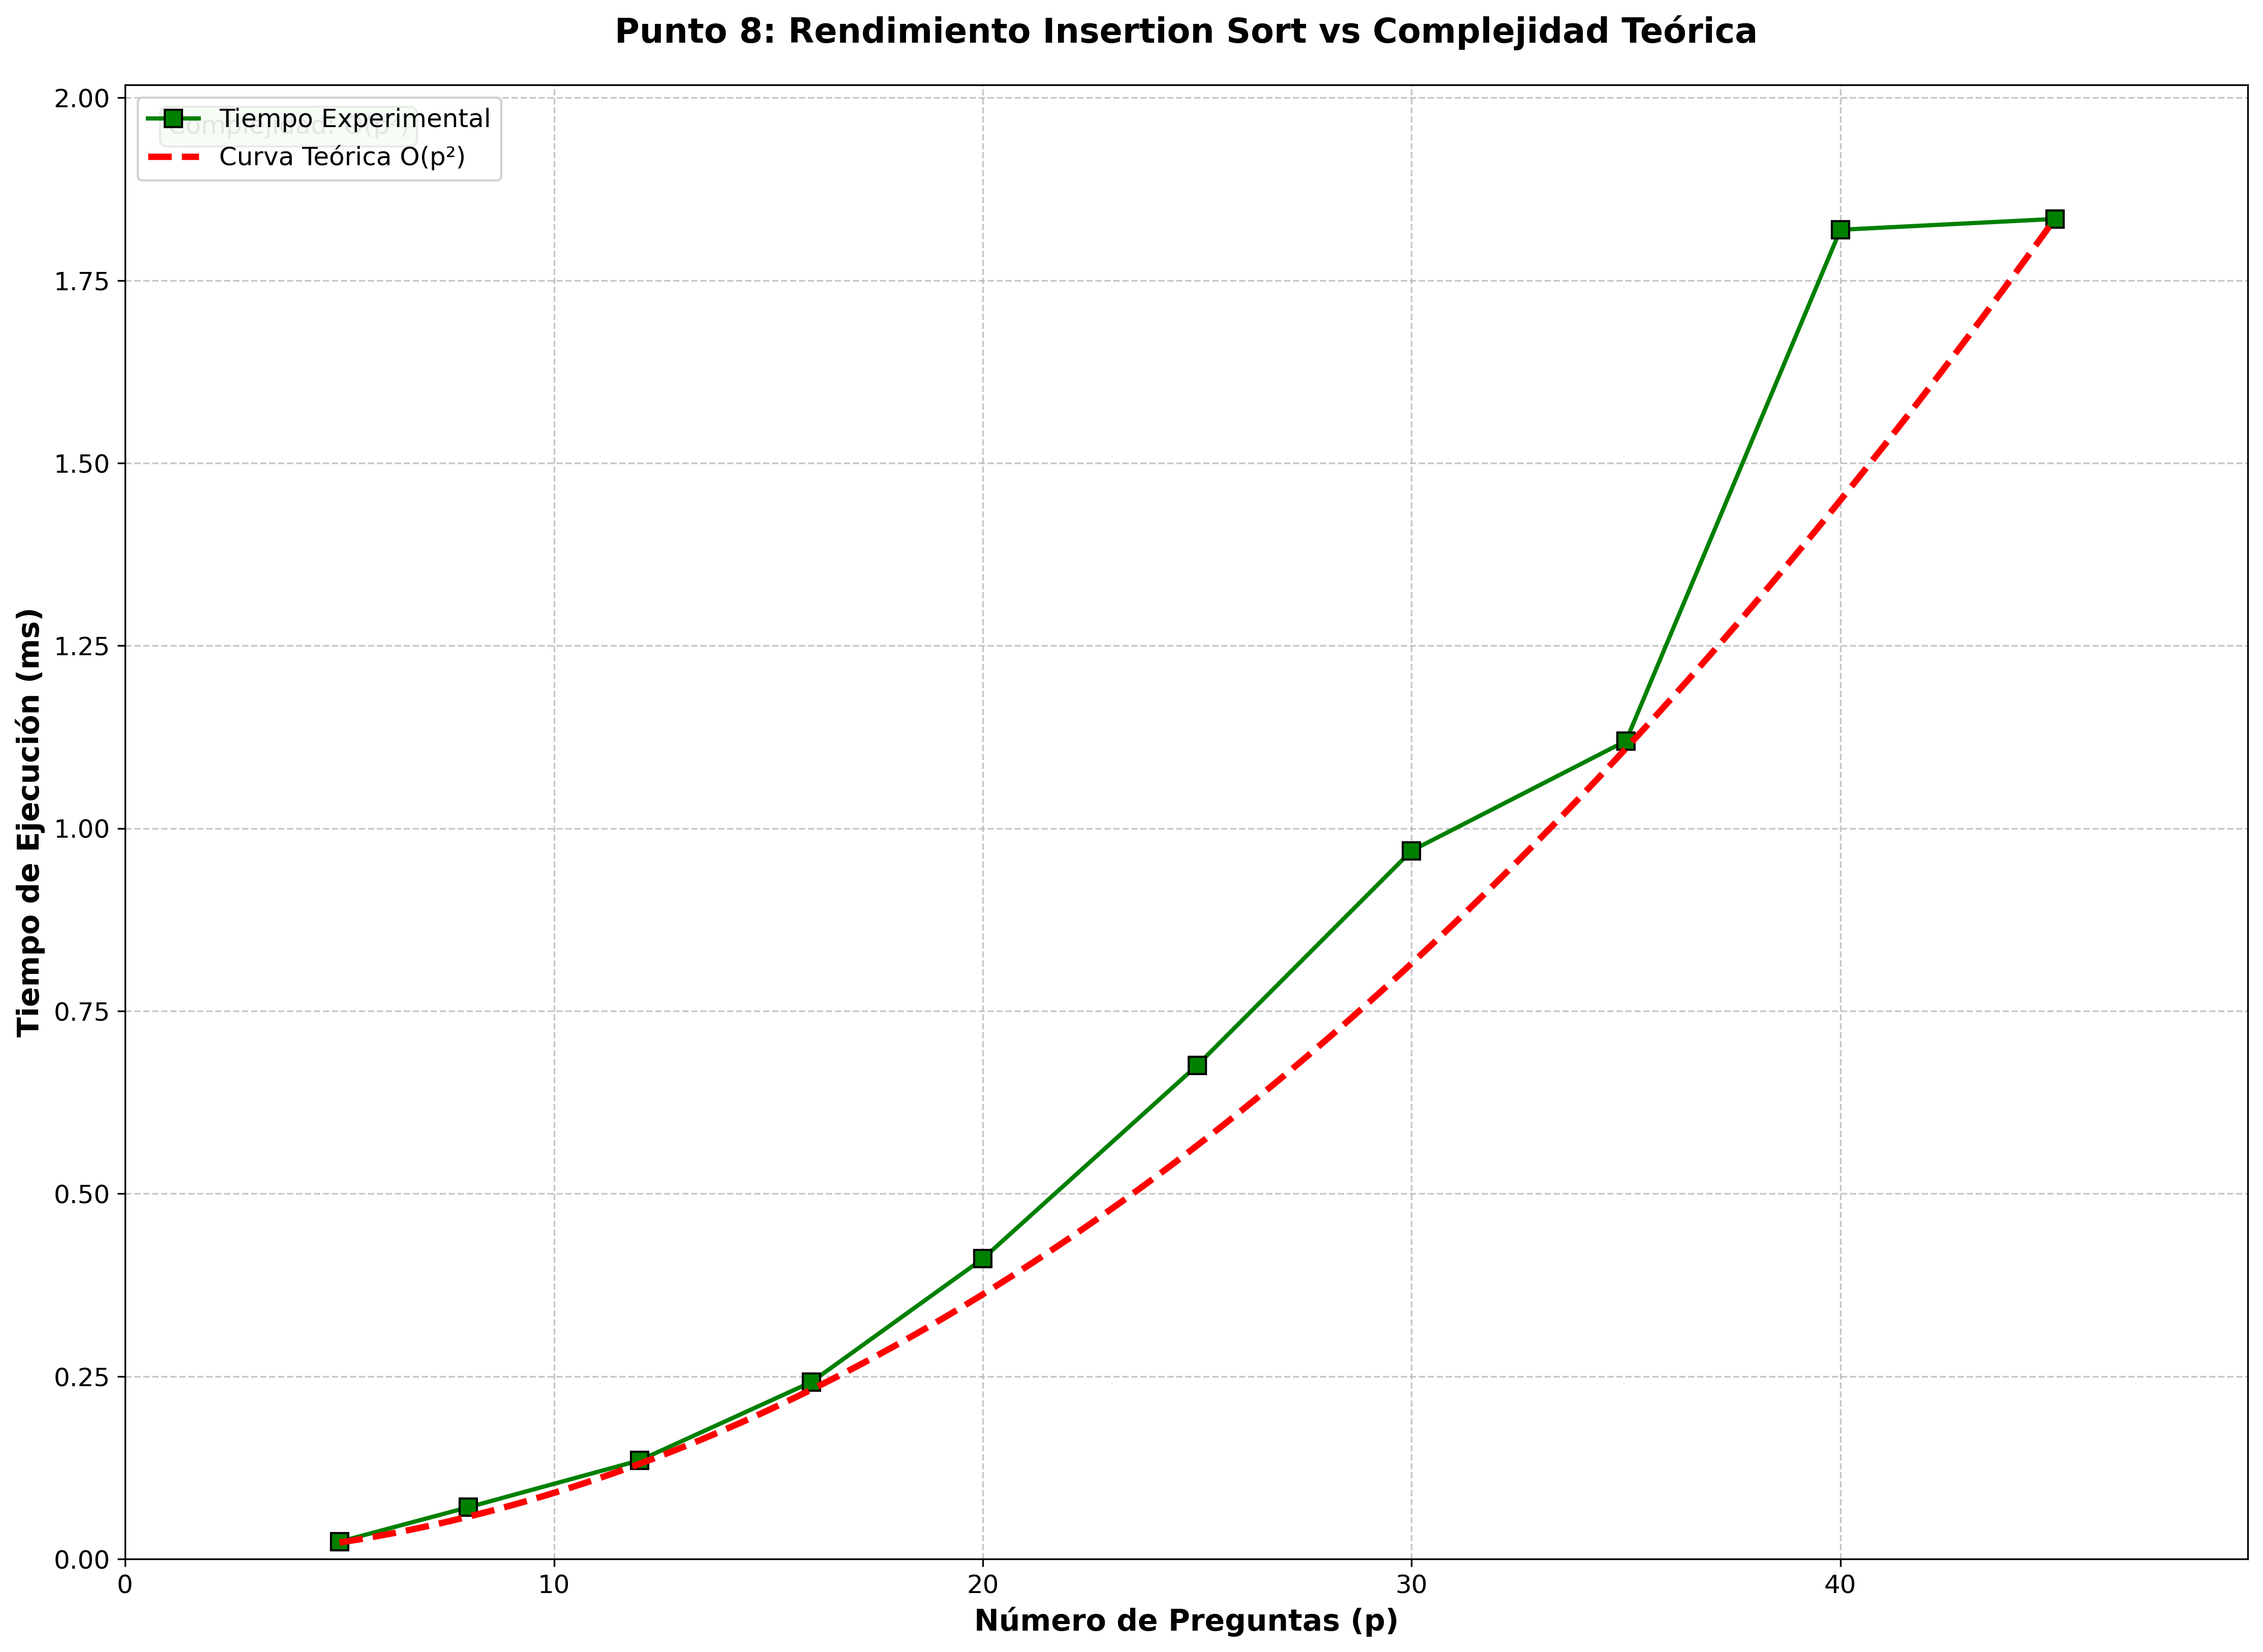
\includegraphics[width=0.8\textwidth]{grafica_punto8_mejorada.png}
\caption{Rendimiento del Insertion Sort vs Complejidad Teórica O(p²)}
\label{fig:insertion_sort_p8}
\end{figure}

La Figura \ref{fig:insertion_sort_p8} muestra claramente el crecimiento cuadrático del tiempo de ejecución conforme aumenta el número de preguntas, validando la complejidad teórica O(p²).

\subsection{Punto 12: Insertion Sort Optimizado - Complejidad O(p²)}

El algoritmo optimizado del Punto 12 mantiene la misma complejidad O(p²) pero con una constante menor, resultando en tiempos de ejecución más eficientes:

\begin{figure}[h]
\centering
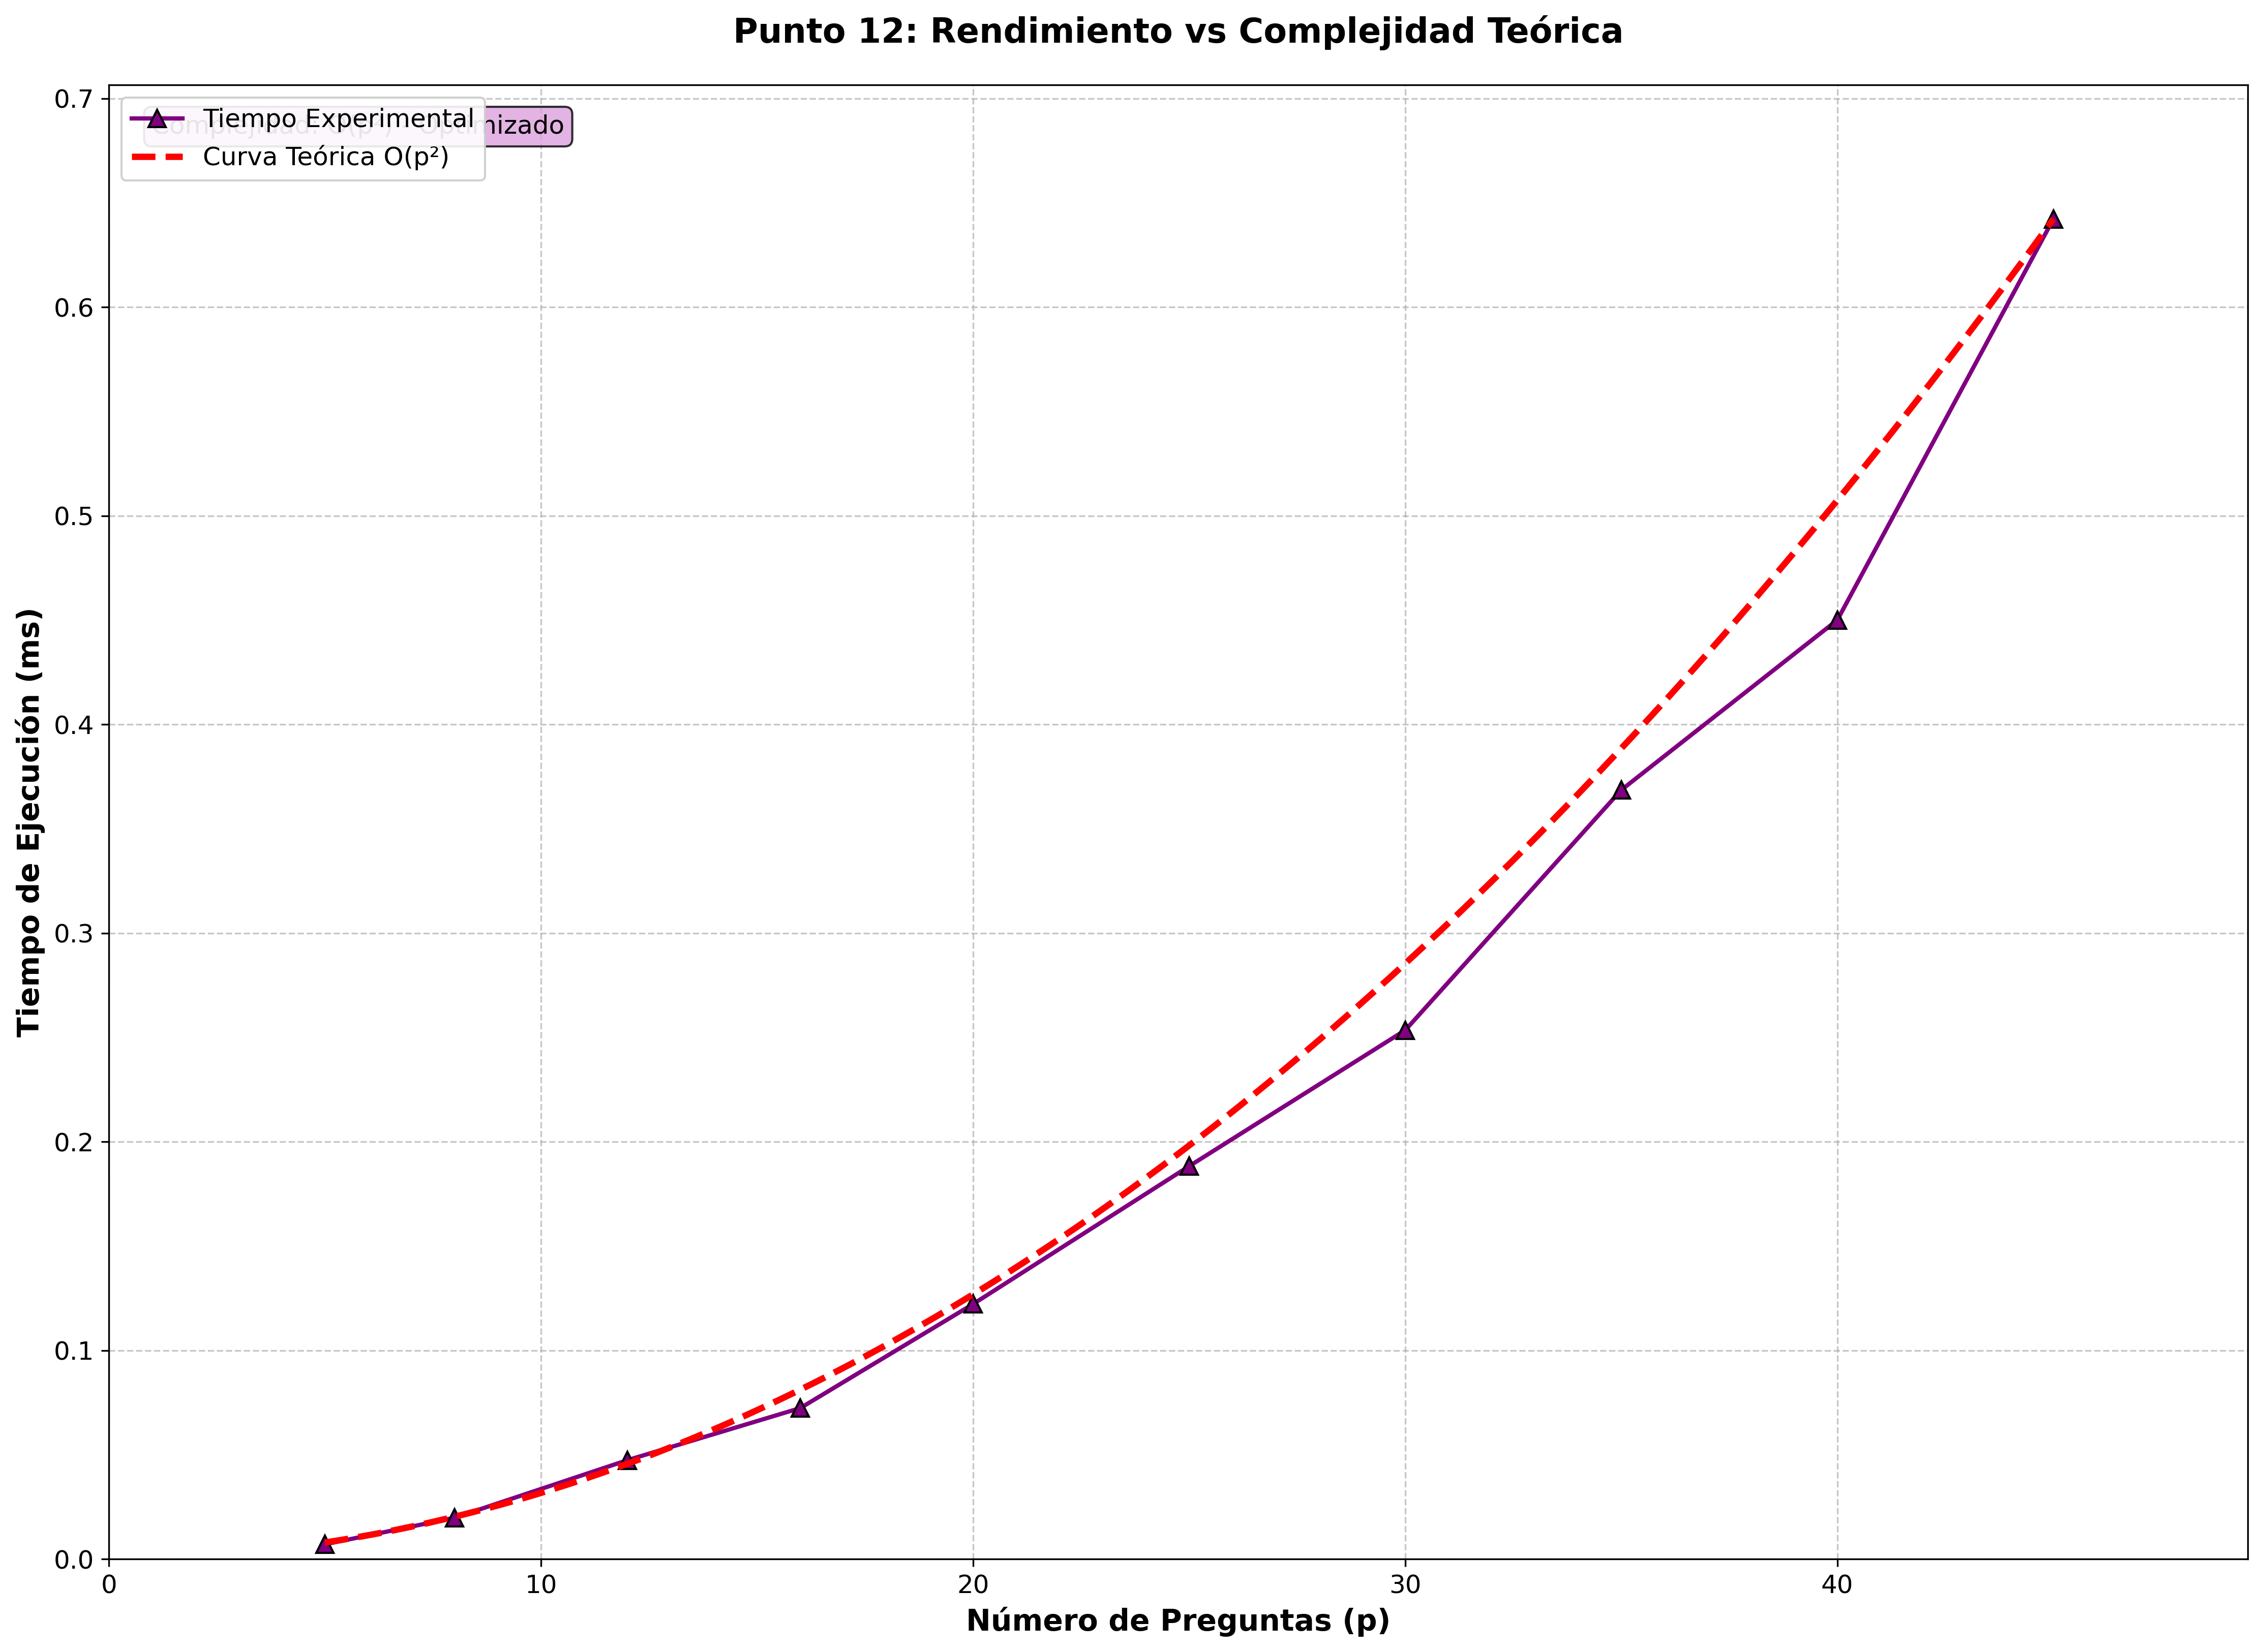
\includegraphics[width=0.8\textwidth]{grafica_punto12_mejorada.png}
\caption{Rendimiento del Insertion Sort Optimizado vs Complejidad Teórica O(p²)}
\label{fig:insertion_sort_p12}
\end{figure}

Como se observa en la Figura \ref{fig:insertion_sort_p12}, aunque la complejidad sigue siendo O(p²), la optimización reduce significativamente el tiempo de ejecución en comparación con la implementación del Punto 8.

\subsection{Comparación de Algoritmos}

La siguiente gráfica presenta una comparación directa de los tres algoritmos analizados:

\begin{figure}[h]
\centering
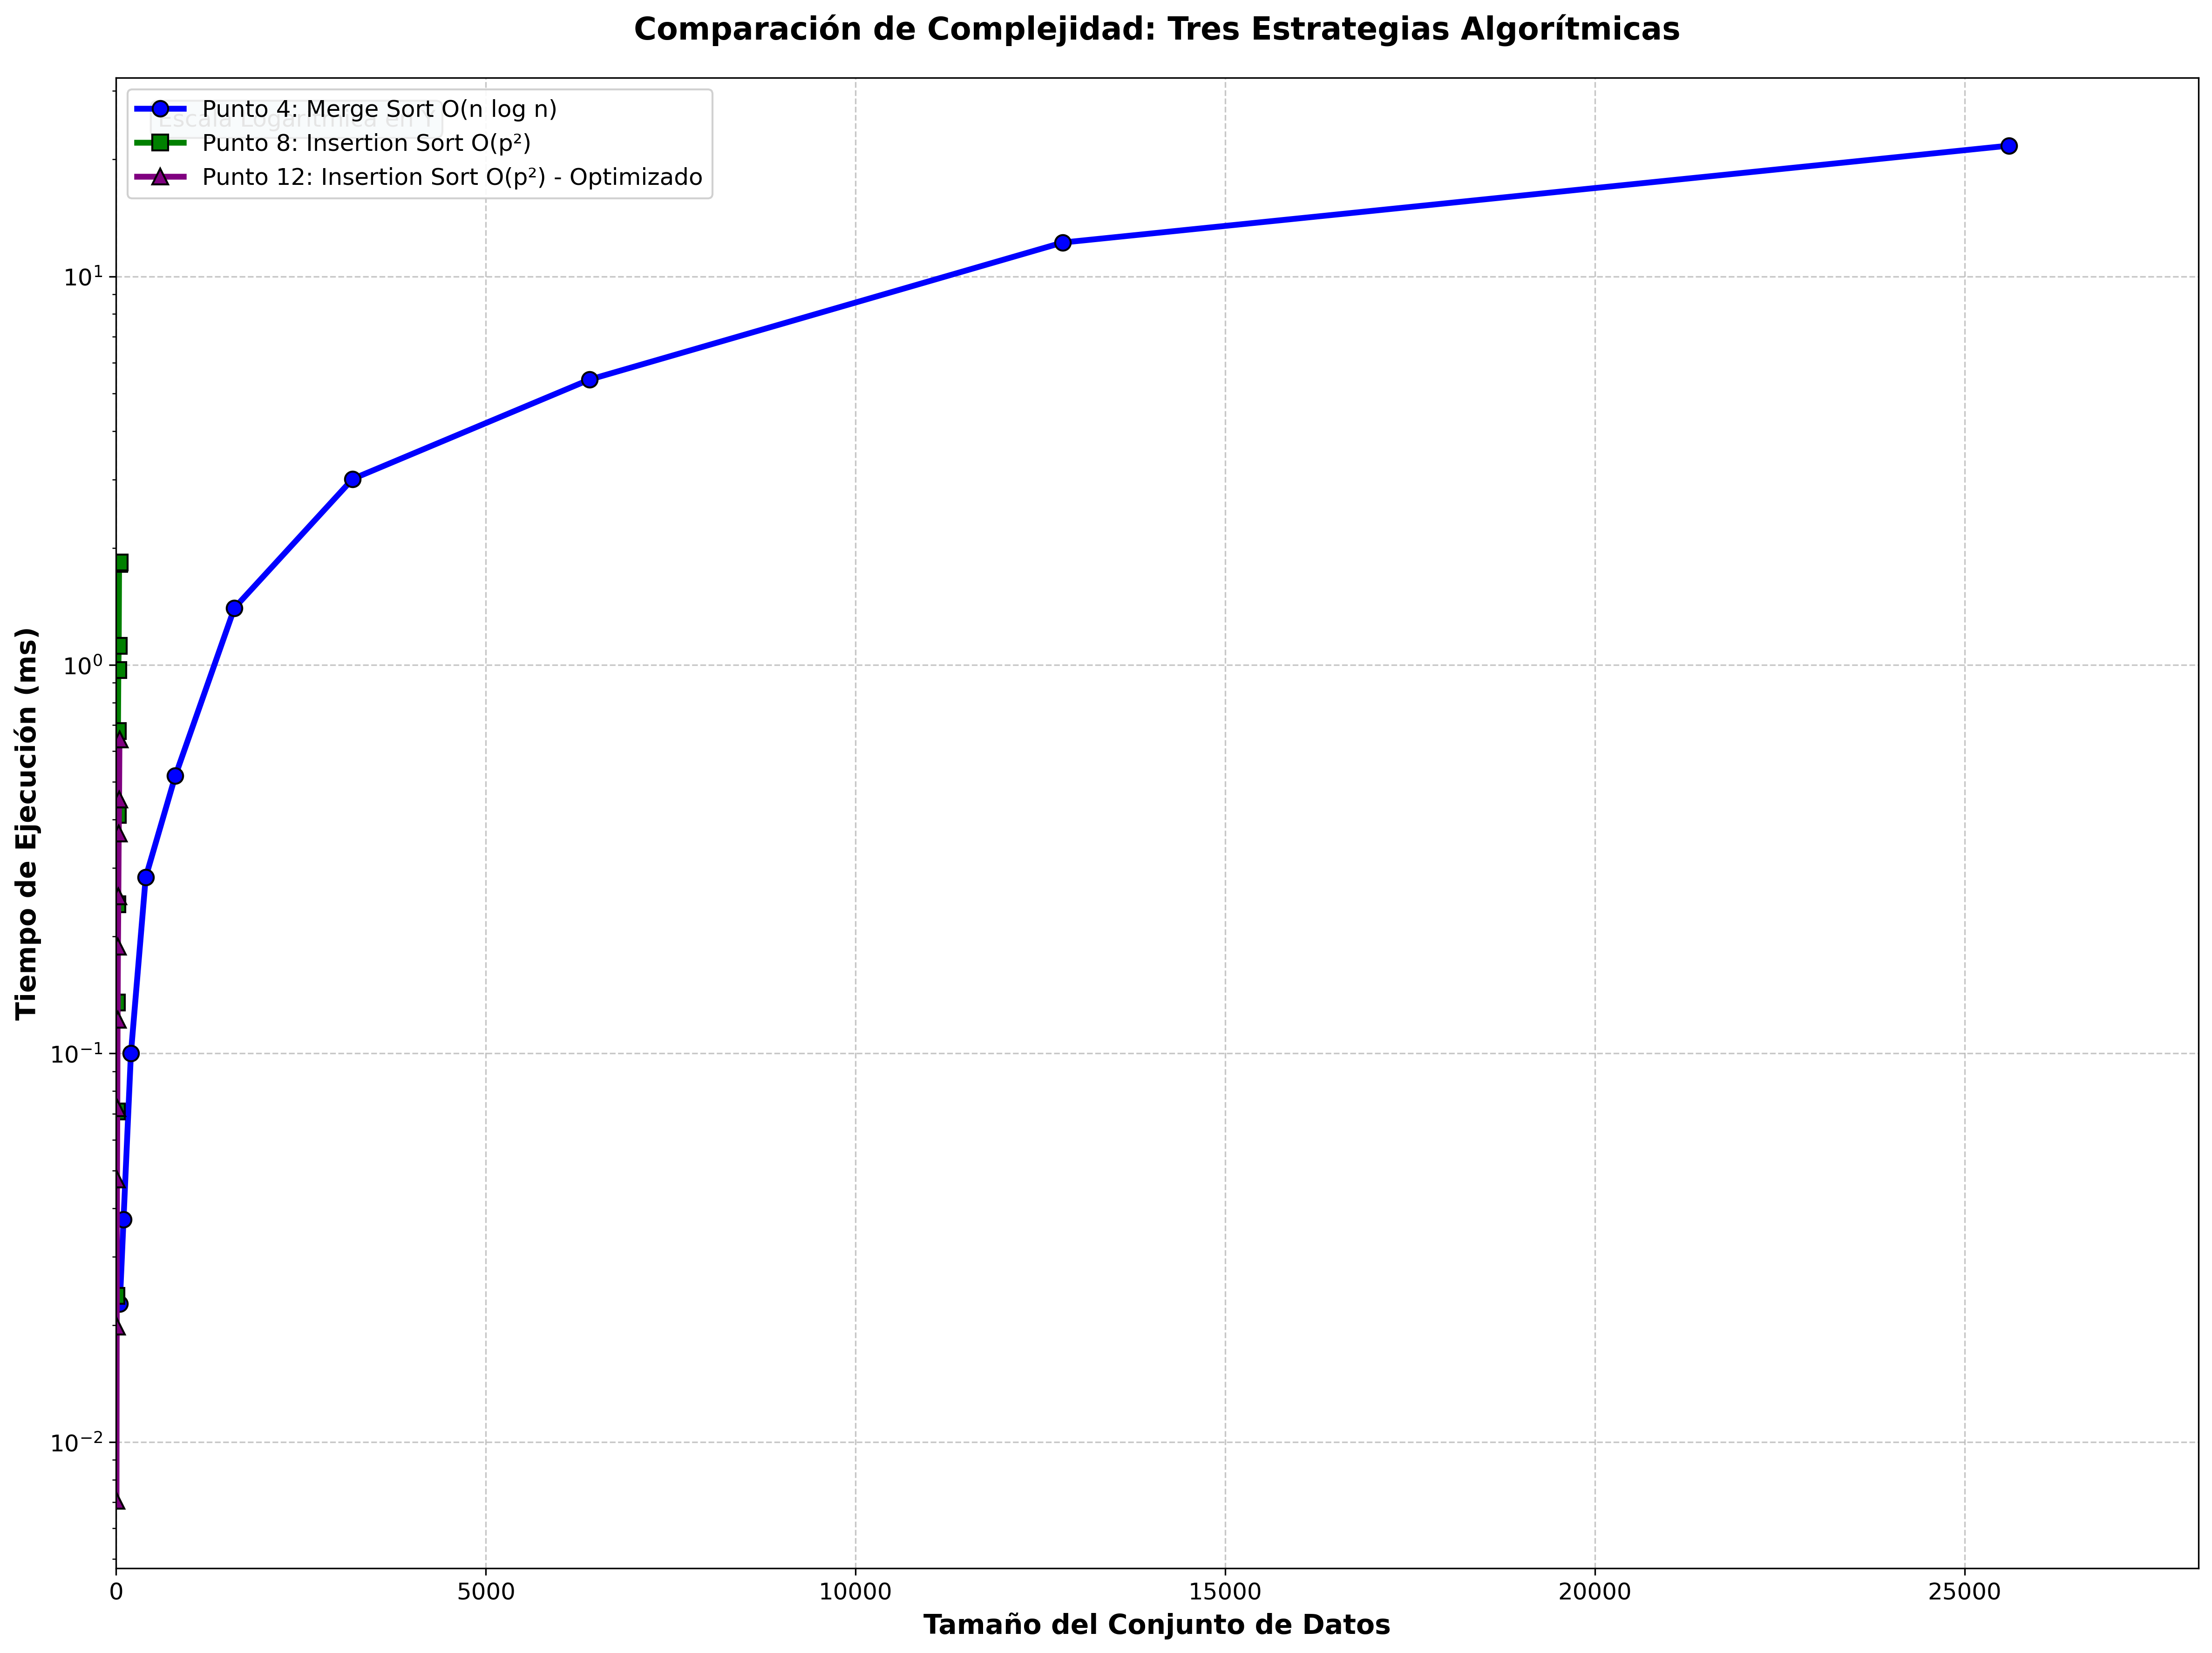
\includegraphics[width=0.9\textwidth]{grafica_comparativa_mejorada.png}
\caption{Comparación de Complejidad: Tres Estrategias Algorítmicas}
\label{fig:comparacion_algoritmos}
\end{figure}

La Figura \ref{fig:comparacion_algoritmos} utiliza una escala logarítmica en el eje Y para mostrar claramente las diferencias en el crecimiento de los tiempos de ejecución:

\begin{itemize}
    \item \textbf{Merge Sort (Punto 4)}: Muestra el crecimiento más lento, característico de O(n log n)
    \item \textbf{Insertion Sort (Punto 8)}: Presenta crecimiento cuadrático O(p²)
    \item \textbf{Insertion Sort Optimizado (Punto 12)}: Mantiene O(p²) pero con mejor rendimiento
\end{itemize}

\subsection{Conclusiones del Análisis}

Los resultados experimentales confirman las complejidades teóricas de los algoritmos implementados:

\begin{enumerate}
    \item El Merge Sort del Punto 4 mantiene su complejidad O(n log n) de manera consistente
    \item Los algoritmos de Insertion Sort de los Puntos 8 y 12 confirman la complejidad O(p²)
    \item Las optimizaciones en el Punto 12 resultan en mejor rendimiento sin cambiar la complejidad asintótica
    \item Para conjuntos de datos grandes, el Merge Sort es significativamente más eficiente que los algoritmos cuadráticos
\end{enumerate}

Este análisis experimental valida la correcta implementación de los algoritmos y proporciona evidencia empírica de sus características de complejidad computacional.

